% Technische Mini-Dokumentation: Ladezeit einer Website
% Kompilieren: pdflatex main -> bibtex main -> pdflatex main (2x)
%              oder einfach: latexmk -pdf main
\documentclass[11pt,a4paper]{article}

\usepackage[T1]{fontenc}
\usepackage{lmodern}
\usepackage[ngerman,provide=*]{babel} % deutsche Silbentrennung und Bezeichner
\usepackage[margin=2.5cm]{geometry}
\usepackage{amsmath}
\usepackage{siunitx}
\sisetup{locale=DE, per-mode=symbol}
\usepackage{booktabs}
\usepackage{caption}
\captionsetup{font=small, labelfont=bf}
\usepackage{tikz}
\usetikzlibrary{arrows.meta}
\usepackage[hidelinks]{hyperref}
\hyphenation{Glei-chung Dar-stel-lung}

\title{Ladezeit einer Website:\\ vom Seitenaufruf bis zur Darstellung}
\author{Technische Mini-Dokumentation}
\date{12.~November 2026}

\begin{document}
\maketitle

% Abschnitt 1: Einleitung
\section{Einleitung}
\label{sec:einleitung}

Die Ladezeit entscheidet mit darüber, ob Besucherinnen und Besucher auf einer
Website bleiben. Sie hängt nicht nur von der Geschwindigkeit des Servers ab,
sondern auch von der Zahl der Netzwerkschritte und von der Datenmenge, die der
Browser übertragen muss. Diese Dokumentation beschreibt den Ablauf eines
Seitenaufrufs, stellt ein einfaches Modell für die Ladezeit auf und wendet es
auf eine Beispielseite an. Grundlage für den Datenaustausch zwischen Browser
und Webserver ist das Protokoll HTTP, dessen Bedeutung der Nachrichten in
RFC~9110 festgelegt ist~\cite{rfc9110}.

% Abschnitt 2 und 2.1: Ablauf eines Seitenaufrufs (mit Abbildung)
\section{Vom Seitenaufruf zur Antwort}
\label{sec:ablauf}

\subsection{Ablauf eines Seitenaufrufs}
\label{sec:schritte}

Abbildung~\ref{fig:ablauf} zeigt die Schritte, die nach Eingabe einer Adresse
ablaufen. Zuerst ermittelt der Browser über einen DNS-Server die IP-Adresse
des Webservers. Danach baut er eine Verbindung auf und sendet eine Anfrage mit
der Methode \texttt{GET}. Der Server antwortet mit einem Statuscode, etwa
\texttt{200} bei Erfolg oder \texttt{404} bei einer nicht gefundenen
Ressource~\cite{rfc9110}, und liefert das HTML-Dokument. Für jede darin
eingebundene Datei (Stylesheets, Skripte, Bilder) folgt eine weitere Anfrage.

\begin{figure}[htb]
  \centering
  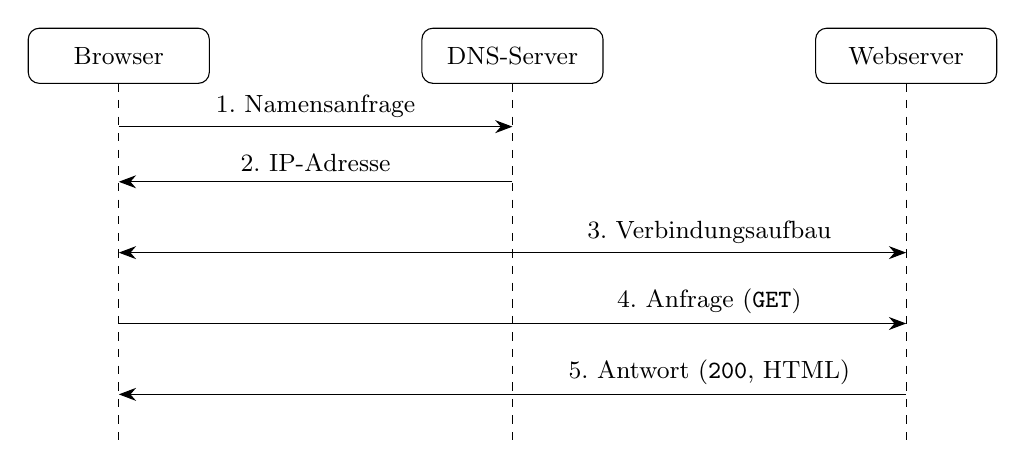
\begin{tikzpicture}[>={Stealth[length=2.2mm]}, font=\small]
    % Teilnehmer
    \foreach \x/\name in {0/Browser, 5/DNS-Server, 10/Webserver} {
      \node[draw, rounded corners, minimum width=2.3cm, minimum height=0.7cm]
        at (\x,0) {\name};
      \draw[dashed] (\x,-0.35) -- (\x,-4.9);
    }
    % Nachrichten
    \draw[->] (0,-0.9) -- node[above] {1. Namensanfrage} (5,-0.9);
    \draw[->] (5,-1.6) -- node[above] {2. IP-Adresse} (0,-1.6);
    \draw[<->] (0,-2.5) -- node[above, pos=0.75] {3. Verbindungsaufbau} (10,-2.5);
    \draw[->] (0,-3.4) -- node[above, pos=0.75] {4. Anfrage (\texttt{GET})} (10,-3.4);
    \draw[->] (10,-4.3) -- node[above, pos=0.25] {5. Antwort (\texttt{200}, HTML)} (0,-4.3);
  \end{tikzpicture}
  \caption{Ablauf eines Seitenaufrufs zwischen Browser, DNS-Server und
           Webserver (eigene Darstellung).}
  \label{fig:ablauf}
\end{figure}

% Abschnitt 2.2: Modell für die Ladezeit (mit Gleichung und Aufzählung)
\subsection{Modell für die Ladezeit}
\label{sec:modell}

Fasst man die Schritte aus Abbildung~\ref{fig:ablauf} zusammen, ergibt sich
für die Ladezeit $t_\mathrm{L}$ näherungsweise
\begin{equation}
  t_\mathrm{L} = t_\mathrm{DNS} + t_\mathrm{V} + t_\mathrm{S} + \frac{S}{B}\,.
  \label{eq:ladezeit}
\end{equation}
Dabei ist $t_\mathrm{DNS}$ die Dauer der Namensauflösung, $t_\mathrm{V}$ die
Dauer des Verbindungsaufbaus, $t_\mathrm{S}$ die Bearbeitungszeit des Servers,
$S$ die übertragene Datenmenge und $B$ die Datenrate der Verbindung. Das
Modell vernachlässigt parallele Übertragungen und die Zeit für das Rendern im
Browser, zeigt aber, wo sich ansetzen lässt:
\begin{itemize}
  \item Datenmenge $S$ verringern, etwa durch Komprimierung, moderne
        Bildformate und das Entfernen ungenutzter Skripte.
  \item Wiederholte Übertragungen vermeiden, indem der Browser unveränderte
        Dateien aus dem Cache lädt.
  \item Wartezeiten $t_\mathrm{V}$ und $t_\mathrm{S}$ senken, zum Beispiel
        durch Server in der Nähe der Nutzer und durch vorab erzeugte Seiten.
\end{itemize}


\bibliographystyle{plain}
\bibliography{literatur}

\end{document}
